\documentclass[border=4pt]{standalone}
\usepackage{tikz}
\usetikzlibrary{shapes.geometric,arrows.meta,positioning,calc}
\definecolor{boxblue}{RGB}{225,238,252}
\definecolor{boxgreen}{RGB}{225,247,231}
\definecolor{boxorange}{RGB}{253,236,216}
\definecolor{boxgray}{RGB}{237,237,237}
\begin{document}
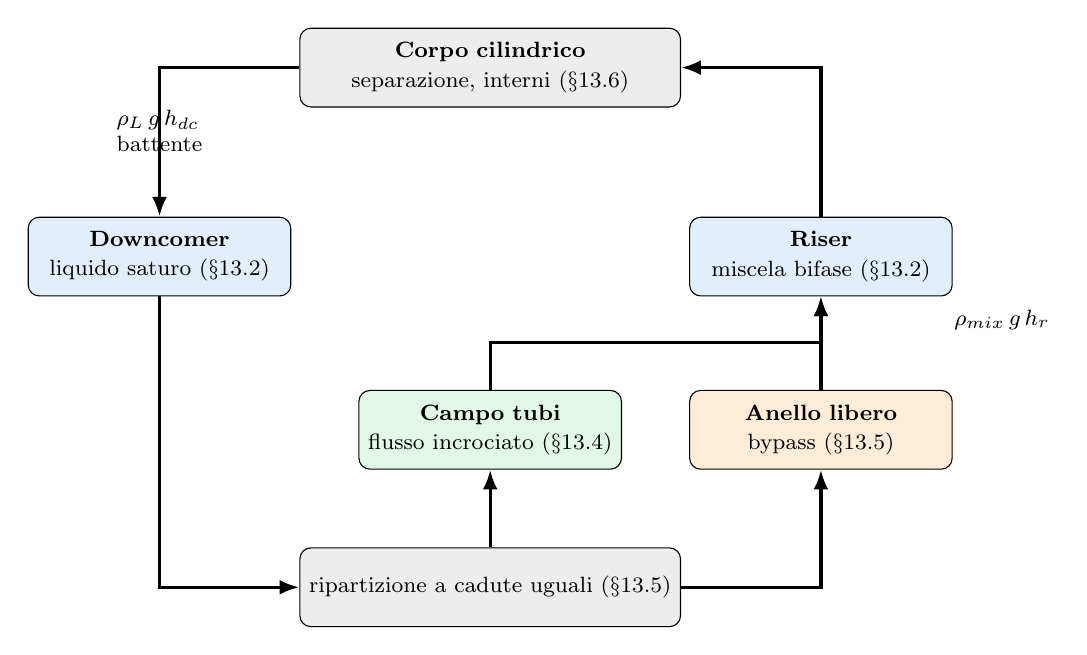
\begin{tikzpicture}[
  box/.style={draw, rectangle, rounded corners, minimum height=1.0cm, text width=3.1cm, align=center, font=\footnotesize},
  arr/.style={-{Latex[length=2.5mm]}, very thick}
]
\node[box, fill=boxgray, text width=4.6cm] (drum) at (0,4.2) {\textbf{Corpo cilindrico}\\[1pt]separazione, interni ($\S13.6$)};
\node[box, fill=boxblue] (dc) at (-4.2,1.8) {\textbf{Downcomer}\\[1pt]liquido saturo ($\S13.2$)};
\node[box, fill=boxgreen] (bundle) at (0,-0.4) {\textbf{Campo tubi}\\[1pt]flusso incrociato ($\S13.4$)};
\node[box, fill=boxorange] (ann) at (4.2,-0.4) {\textbf{Anello libero}\\[1pt]bypass ($\S13.5$)};
\node[box, fill=boxblue] (riser) at (4.2,1.8) {\textbf{Riser}\\[1pt]miscela bifase ($\S13.2$)};
\node[box, fill=boxgray, text width=4.6cm] (split) at (0,-2.4) {ripartizione a cadute uguali ($\S13.5$)};

\draw[arr] (drum.west) -| (dc.north);
\draw[arr] (dc.south) |- (split.west);
\draw[arr] (split.north) -- (bundle.south);
\draw[arr] (split.east) -| (ann.south);
\draw[arr] (bundle.north) -- ++(0,0.6) -| (riser.south);
\draw[arr] (ann.north) -- (riser.south);
\draw[arr] (riser.north) |- (drum.east);

\node[font=\footnotesize, align=left] at (-4.2,3.4) {$\rho_L\,g\,h_{dc}$\\ battente};
\node[font=\footnotesize, align=left] at (6.5,1.0) {$\rho_{mix}\,g\,h_{r}$};
\end{tikzpicture}
\end{document}
